\documentclass{beamer}

% Theme
\usetheme{Madrid}
\usecolortheme{default}

% Packages
\usepackage{amsmath,amssymb,amsfonts}
\usepackage{graphicx}
\usepackage{xcolor}
\usepackage{tikz}
\usepackage{tkz-euclide}
\usepackage{array}
\usepackage{multirow}
\usepackage{longtable}
\usepackage{lscape}
\usepackage{listings}
\lstset{
    basicstyle=\ttfamily\small,
    keywordstyle=\color{blue},
    commentstyle=\color{gray},
    stringstyle=\color{red},
    showstringspaces=false,
    breaklines=true
}



% Custom macros
\newcommand{\myvec}[1]{\begin{pmatrix}#1\end{pmatrix}}
\newcommand{\brak}[1]{\left( #1 \right)}

% Redefine \vec to bold letters only (no arrow)
\renewcommand{\vec}[1]{\mathbf{#1}}

\title{4.6.7}
\author{EE25BTECH11019 -- Darji Vivek M.}
\date{}


\begin{document}

\begin{frame}
\titlepage
\end{frame}

%-------------------------------
\begin{frame}{Question}
\textbf{Question}:\\
Find the equation of the line which passes through the point $(3,4,5)$ and is parallel to the vector $2\vec{i}+\vec{j}-3\vec{k}$.\\[4pt]
\hfill $\brak{12,2018}$
\end{frame}

%-------------------------------
\begin{frame}{Solution}

\textbf{Matrix Method:}\\
Let the point be
\begin{align}
\vec{A}=\myvec{3\\4\\5},
\end{align}
and the direction vector be
\begin{align}
\vec{d}=\myvec{2\\1\\-3}.
\end{align}
\end{frame}

%-------------------------------
\begin{frame}{Solution}
The general form of a line is
\begin{align}
\vec{r}=\vec{A}+\lambda\vec{d}.
\end{align}

Substituting values,
\begin{align}
\vec{r}=\myvec{3\\4\\5}+\lambda\myvec{2\\1\\-3}.
\end{align}

\begin{align}
\vec{r}={\myvec{3+2\lambda\\4+\lambda\\5-3\lambda}}
\end{align}
Equation of line in symmetric form

\begin{align}
\frac{x-3}{2}=\frac{y-4}{1}=\frac{z-5}{-3}
\end{align}
\end{frame}

%-------------------------------
\begin{frame}[fragile]{C Code}
\begin{lstlisting}
#include<stdio.h>

void line_point(double lambda, double *out) {
    // Line: r = A + lambda*d
    double A[3] = {3.0, 4.0, 5.0};
    double d[3] = {2.0, 1.0, -3.0};

    for(int i=0; i<3; i++) {
        out[i] = A[i] + lambda * d[i];
    }
}
\end{lstlisting}
\end{frame}
%-------------------------------
\begin{frame}[fragile]{Python (Call)}
\begin{lstlisting}[language=Python]
import ctypes
import numpy as np
import matplotlib.pyplot as plt

# Load shared library
lib = ctypes.CDLL("./7.so")
lib.line_point.argtypes = [ctypes.c_double, np.ctypeslib.ndpointer(dtype=np.float64)]
lib.line_point.restype = None

def line_point(lambda_val):
    out = np.zeros(3, dtype=np.float64)
    lib.line_point(lambda_val, out)
    return out

# Generate line points
lambdas = np.linspace(-5, 5, 50)
points = np.array([line_point(l) for l in lambdas])
\end{lstlisting}
\end{frame}

\begin{frame}[fragile]{Python (Plot)}
\begin{lstlisting}[language=Python]
# Given point A
A = np.array([3, 4, 5])

# Plot
fig = plt.figure()
ax = fig.add_subplot(111, projection='3d')

ax.plot(points[:,0], points[:,1], points[:,2], label="Line")
ax.scatter(A[0], A[1], A[2], color='red', s=50, label="Point A (3,4,5)")

# Annotate the point
ax.text(A[0], A[1], A[2], "A(3,4,5)", fontsize=10, color='red')

ax.set_xlabel("X")
ax.set_ylabel("Y")
ax.set_zlabel("Z")
ax.legend()
plt.show()

\end{lstlisting}
\end{frame}

\begin{frame}{Python Output and Plot}
\begin{figure}[h!]
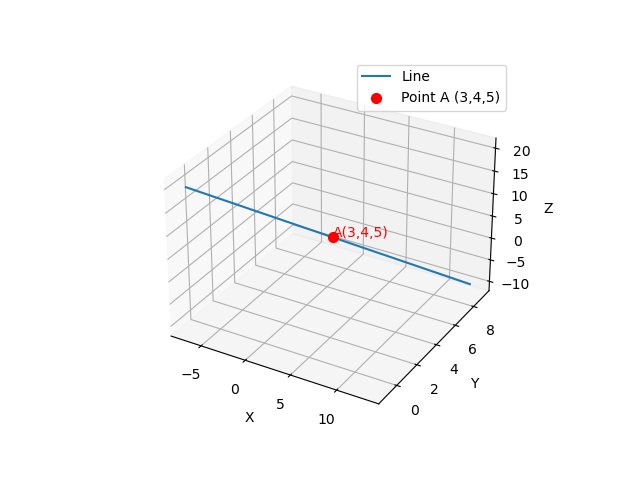
\includegraphics[width=0.75\columnwidth]{figs/7.png}
\caption{Line through $\vec{A}$ parallel to $\vec{d}$}
\end{figure}
\end{frame}

\end{document}
